% LeBlanc v4 project report (follows the format of the 22 August 2026 progress report).
% Numbers come from ../paper/numbers.json and ../paper/numbers.tex (generated from run/leblanc.db).
% Build: pdflatex leblanc_report.tex (twice).
\documentclass[11pt]{article}
\usepackage[margin=1in]{geometry}
\usepackage{graphicx}
\usepackage{booktabs}
\usepackage{float}
\usepackage{xcolor}
\usepackage{enumitem}
\usepackage[hidelinks]{hyperref}
\usepackage{caption}
\usepackage{tikz}
\usetikzlibrary{arrows.meta,positioning,fit}
\captionsetup{font=small,labelfont=bf}
\setlist{itemsep=2pt}
% generated by paper/make_figures.py from the run database; do not edit
\newcommand{\NTasks}{56}
\newcommand{\NCwe}{38}
\newcommand{\NSpValid}{45}
\newcommand{\Reps}{3}
\newcommand{\Temp}{0.7}
\newcommand{\Effort}{low}
\newcommand{\MaxTok}{16{,}384}
\newcommand{\MaxRounds}{3}
\newcommand{\GenericLine}{Write secure code and avoid common security vulnerabilities.}
\newcommand{\NCells}{2{,}520}
\newcommand{\NCalls}{2{,}098}
\newcommand{\TotalCost}{0.78}
\newcommand{\RunMinutes}{39}
\newcommand{\Kappa}{0.004}


\title{LeBlanc: Re-evaluating Security Scaffolding for Contemporary Code LLMs\\[0.4em]
\large B.Tech Capstone Project Report: System, Study and Results}
\author{6 November 2026 \;--\; Suryanshu Banerjee, Ayushi Ranjan, Swadha Kumari, Vraj Soni\\
\small Supervisor: Prof.\ Deepti Patole}
\date{}

\begin{document}
\maketitle

\begin{abstract}
LeBlanc is a research platform and Model Context Protocol (MCP) tool that measures whether two common ways of making
LLM-written code safer, a security instruction in the prompt and scanner-guided repair, still help on current
models, and what they cost. Since the August report the system was rebuilt from scratch (v4) to remove the design
problems the pilot exposed, and the full study has been run: 56 validated tasks with executable functional and
security tests, three current models, three prompt arms, three fix strategies and three repetitions, \NCells{}
scored outputs, for \$\TotalCost{} in API usage. The main findings are that static analysers flag far fewer outputs
than fail the security tests and barely agree with them, that scanner-guided repair satisfies the analysers without
changing tested security, and that a one-line security preamble is the only intervention with a clear benefit, on
two of the three models. The software, the MCP server, the run database and a draft paper are complete.
\end{abstract}

\section{Outcome in one page}
\begin{itemize}
\item \textbf{Built:} a resumable experiment runner, a three-way judge (Bandit and Semgrep, the dataset's security
      tests, its functional tests), a network-isolated sandbox, a web interface, an MCP server with eight tools and
      a command-line interface. Fifteen self-checks and twelve unit tests pass.
\item \textbf{Run:} 2{,}520 of 2{,}520 planned cells completed with no failed cell, \NCalls{} model calls,
      \RunMinutes{} minutes, \$\TotalCost{}.
\item \textbf{Finding 1:} unaided, the scanners flagged 12.5--13.1\% of outputs, but 54.1--60.7\% failed the task's
      security test; scanner and test verdicts are unrelated (Cohen's $\kappa=\Kappa$).
\item \textbf{Finding 2:} scanner-guided repair raised the scanner-clean rate to 97.6--100\% and changed the
      secure-and-working rate by 0.0 points on every model.
\item \textbf{Finding 3:} a security preamble reduced security-test failures by 11.5 points (Gemini, CWE-specific
      warning) and 11.9 points (DeepSeek, generic line), had no effect on \texttt{gpt-oss-20b}, and did not
      significantly reduce functional correctness on any model.
\item \textbf{Finding 4:} preambles add 9--30 prompt tokens; a blind ``fix vulnerabilities'' pass costs 2.7--4.5 times
      the tokens of the original generation for at most a 3-point gain.
\end{itemize}

\section{What changed since the August report, and why}
The August report proposed a 50-task, six-model study scored by static analysers, with enrichment and repair
applied together. Building and piloting it exposed problems that could not be fixed incrementally, so the system
was rebuilt (v4). Every change is logged with its date and reason in \texttt{docs/DECISIONS.md}.

\begin{table}[H]\centering\small
\begin{tabular}{p{4.3cm}p{5.2cm}p{5.5cm}}
\toprule
Problem found & Evidence & Change in v4\\
\midrule
Only 20 of 50 tasks had functional tests; 13 tasks had a weakness no scanner could see &
Coverage analysis of the v3 dataset & Tasks from CodeSecEval (ISSTA 2026): every task has author-written functional
and security tests\\
62\% of pilot findings were on \texttt{app.run}/\texttt{\_\_main\_\_} boilerplate &
v3 pilot database & System prompt forbids scaffolding; any such finding is flagged and excluded (none occurred)\\
Enrichment always added 4--5 warnings (about 158 tokens, 23\% precise) &
v3 pilot & One-line warnings; generic vs targeted arms; every token counted\\
No control showed whether repair or ``asking again'' helped &
Design review & Blind-repair and resampling controls on the same outputs\\
Groq daily token caps; deprecated model &
Provider documentation & One OpenRouter key, three current models, pinned hosts\\
Some dataset tests swap in fake libraries that accept only the reference's choices &
Stress test before the main run & Such tasks excluded by a fixed rule (56 tasks remain)\\
Published tests demand the reference's exact exception class &
Rehearsal & Lenient scoring primary, published strict scoring always reported\\
\bottomrule
\end{tabular}
\caption{Main design changes. The last two rules were fixed using the dataset's reference solutions only, before
the main run.}
\end{table}

\section{The system}
\subsection{Pipeline}
For each task, model, prompt arm and repetition the runner sends one request, extracts the first Python code
block, and passes the code to the judge. The judge runs Bandit and Semgrep (both must succeed), and the sandbox runs
the task's functional and security tests in a Linux jail with no network, no access to the Windows drives and no
secrets. Repair cells wait for their base output: scanner-guided repair loops up to three rounds; blind repair makes
one call. Every call is logged with tokens, cost, latency, host and finish reason.

\begin{figure}[H]\centering
\resizebox{\textwidth}{!}{% LeBlanc v4 pipeline diagram (TikZ). \input by the paper, the report and the guide.
% Needs \usepackage{tikz} and \usetikzlibrary{arrows.meta,positioning,fit}.
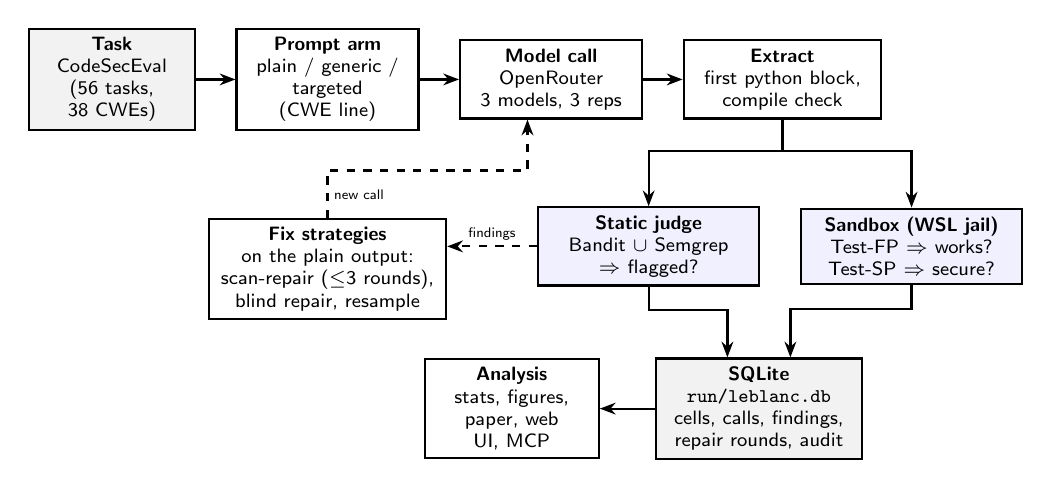
\begin{tikzpicture}[
  font=\sffamily\scriptsize, node distance=4mm and 5mm,
  box/.style={draw, thick, align=center, minimum height=9mm, inner sep=3pt, text width=#1},
  box/.default=19mm,
  data/.style={box=#1, fill=black!5},
  judge/.style={box=#1, fill=blue!6},
  arr/.style={-{Stealth[length=2mm]}, thick},
  lbl/.style={font=\sffamily\tiny, midway, fill=white, inner sep=1pt}]
  % row 1: generation
  \node[data] (task) {\textbf{Task}\\CodeSecEval\\(56 tasks, 38 CWEs)};
  \node[box=21mm, right=of task] (arm) {\textbf{Prompt arm}\\plain / generic /\\targeted (CWE line)};
  \node[box=21mm, right=of arm] (llm) {\textbf{Model call}\\OpenRouter\\3 models, 3 reps};
  \node[box=23mm, right=of llm] (ext) {\textbf{Extract}\\first python block,\\compile check};
  % row 2: judges
  \node[judge=26mm, below=11mm of ext, xshift=-17mm] (sast) {\textbf{Static judge}\\Bandit $\cup$ Semgrep\\$\Rightarrow$ flagged?};
  \node[judge=26mm, right=of sast] (box) {\textbf{Sandbox (WSL jail)}\\Test-FP $\Rightarrow$ works?\\Test-SP $\Rightarrow$ secure?};
  % repair
  \node[box=28mm, below=11mm of arm, xshift=0mm] (rep) {\textbf{Fix strategies}\\on the plain output:\\scan-repair ($\le$3 rounds),\\blind repair, resample};
  % storage and outputs
  \node[data=24mm, below=9mm of sast, xshift=14mm] (db) {\textbf{SQLite} \texttt{run/leblanc.db}\\cells, calls, findings,\\repair rounds, audit};
  \node[box=20mm, left=7mm of db] (out) {\textbf{Analysis}\\stats, figures,\\paper, web UI, MCP};
  \draw[arr] (task) -- (arm);
  \draw[arr] (arm) -- (llm);
  \draw[arr] (llm) -- (ext);
  \draw[arr] (ext.south) -- ++(0,-4mm) -| (sast.north);
  \draw[arr] (ext.south) -- ++(0,-4mm) -| (box.north);
  \draw[arr, dashed] (sast.west) -- node[lbl, above=1pt] {findings} (rep.east |- sast.west);
  \draw[arr, dashed] (rep.north) -- node[lbl, right=1pt] {new call} ++(0,6mm) -| ([xshift=-3mm]llm.south);
  \draw[arr] (sast.south) -- ++(0,-3mm) -| ([xshift=-4mm]db.north);
  \draw[arr] (box.south) -- ++(0,-3mm) -| ([xshift=4mm]db.north);
  \draw[arr] (db.west) -- (out.east);
\end{tikzpicture}
}
\caption{The LeBlanc v4 pipeline, from task to stored, judged output.}
\end{figure}

\subsection{Engineering properties}
\begin{itemize}
\item \textbf{Resumable.} Cells are database rows with leases; a crash or Ctrl-C loses and duplicates nothing.
      Verified by killing a dry run in mid-call and restarting it.
\item \textbf{Balanced under interruption.} Repetition 2 does not start until repetition 1 is finished.
\item \textbf{Cost-safe.} A spend cap stops the run (\$4.50, against \$\TotalCost{} actually used).
\item \textbf{Reproducible.} Pinned dataset revision and hashes, pinned Semgrep rules, seeded task selection, a
      study hash that refuses a database planned under a different configuration, and analyser versions recorded
      on every run.
\item \textbf{Safe.} Model-written code never runs on Windows; the jail is re-verified by the self-check before
      each run.
\end{itemize}

\subsection{Web interface}
Seven pages: Run (start, pause, progress, spend, per-model status), Results (all research questions, computed
live from the database), Runs (every cell, filterable, with a detail page showing the prompt as sent, the code,
findings, repair diffs and test results), Audit (blind false-positive labelling), Dataset (tasks, and a box that
shows what Engine A would add to any prompt), Setup (keys, models, self-check, preflight) and Export.

\begin{figure}[H]\centering
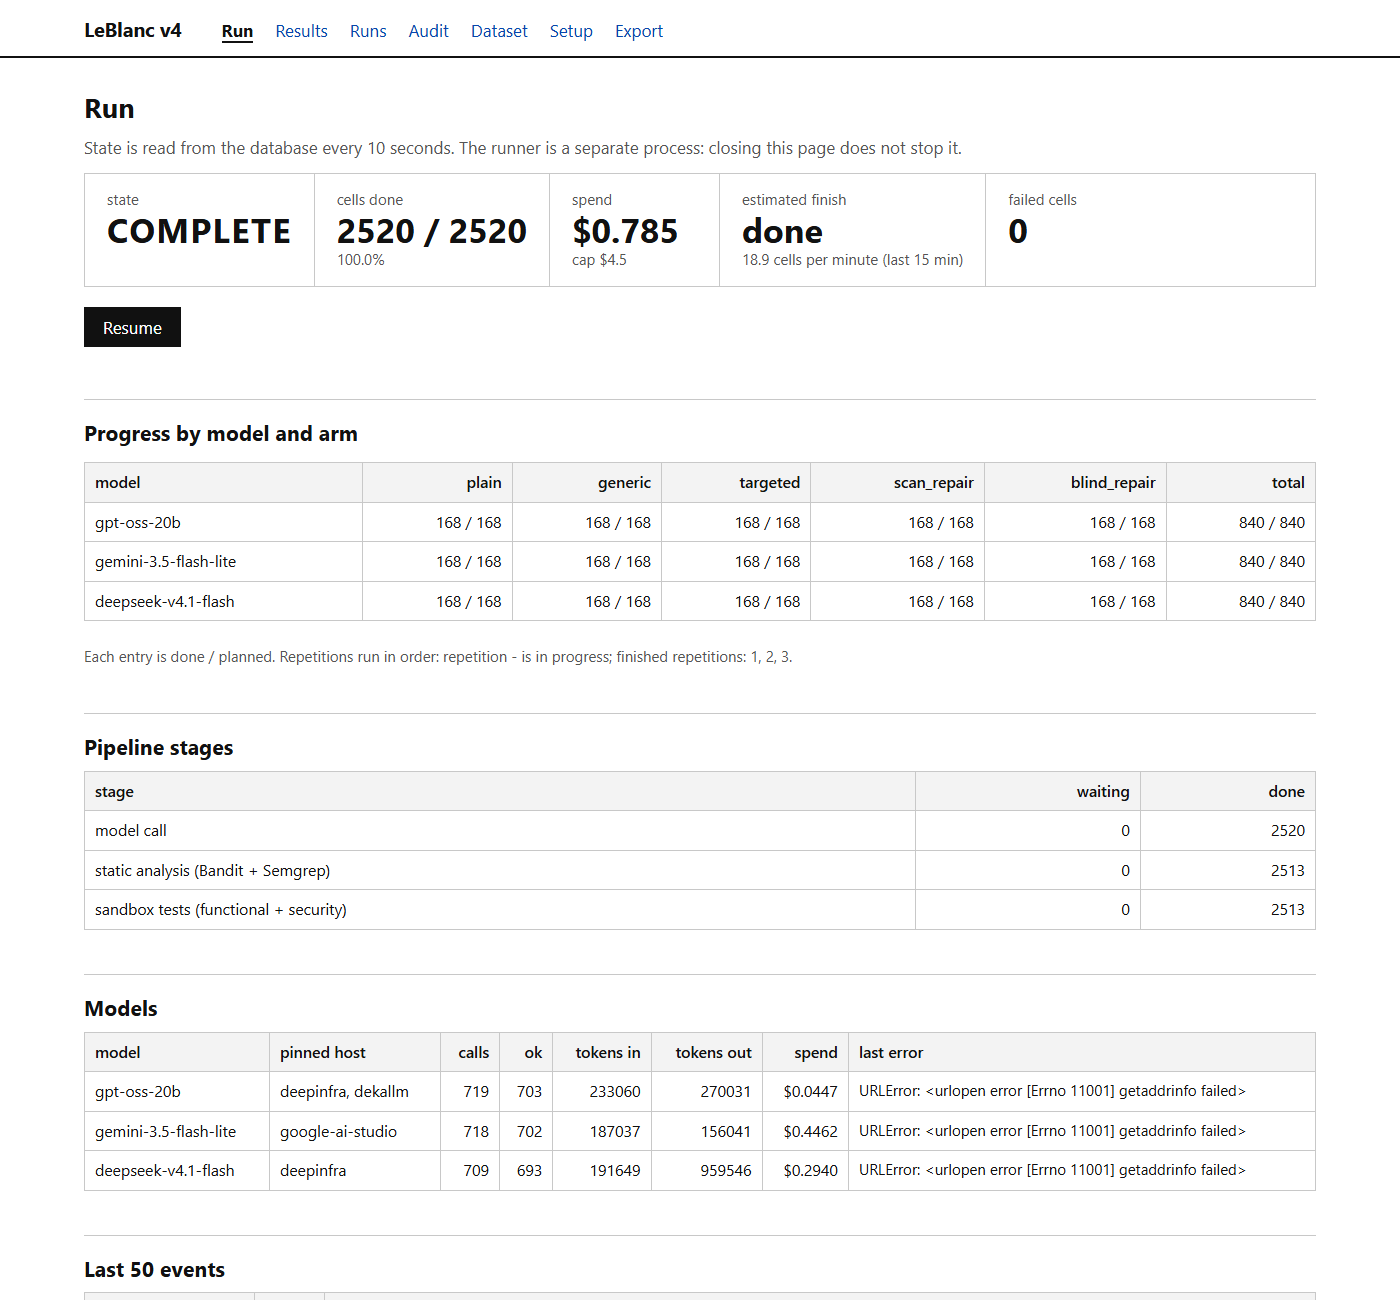
\includegraphics[width=0.49\textwidth]{figures/ui_run.png}\hfill
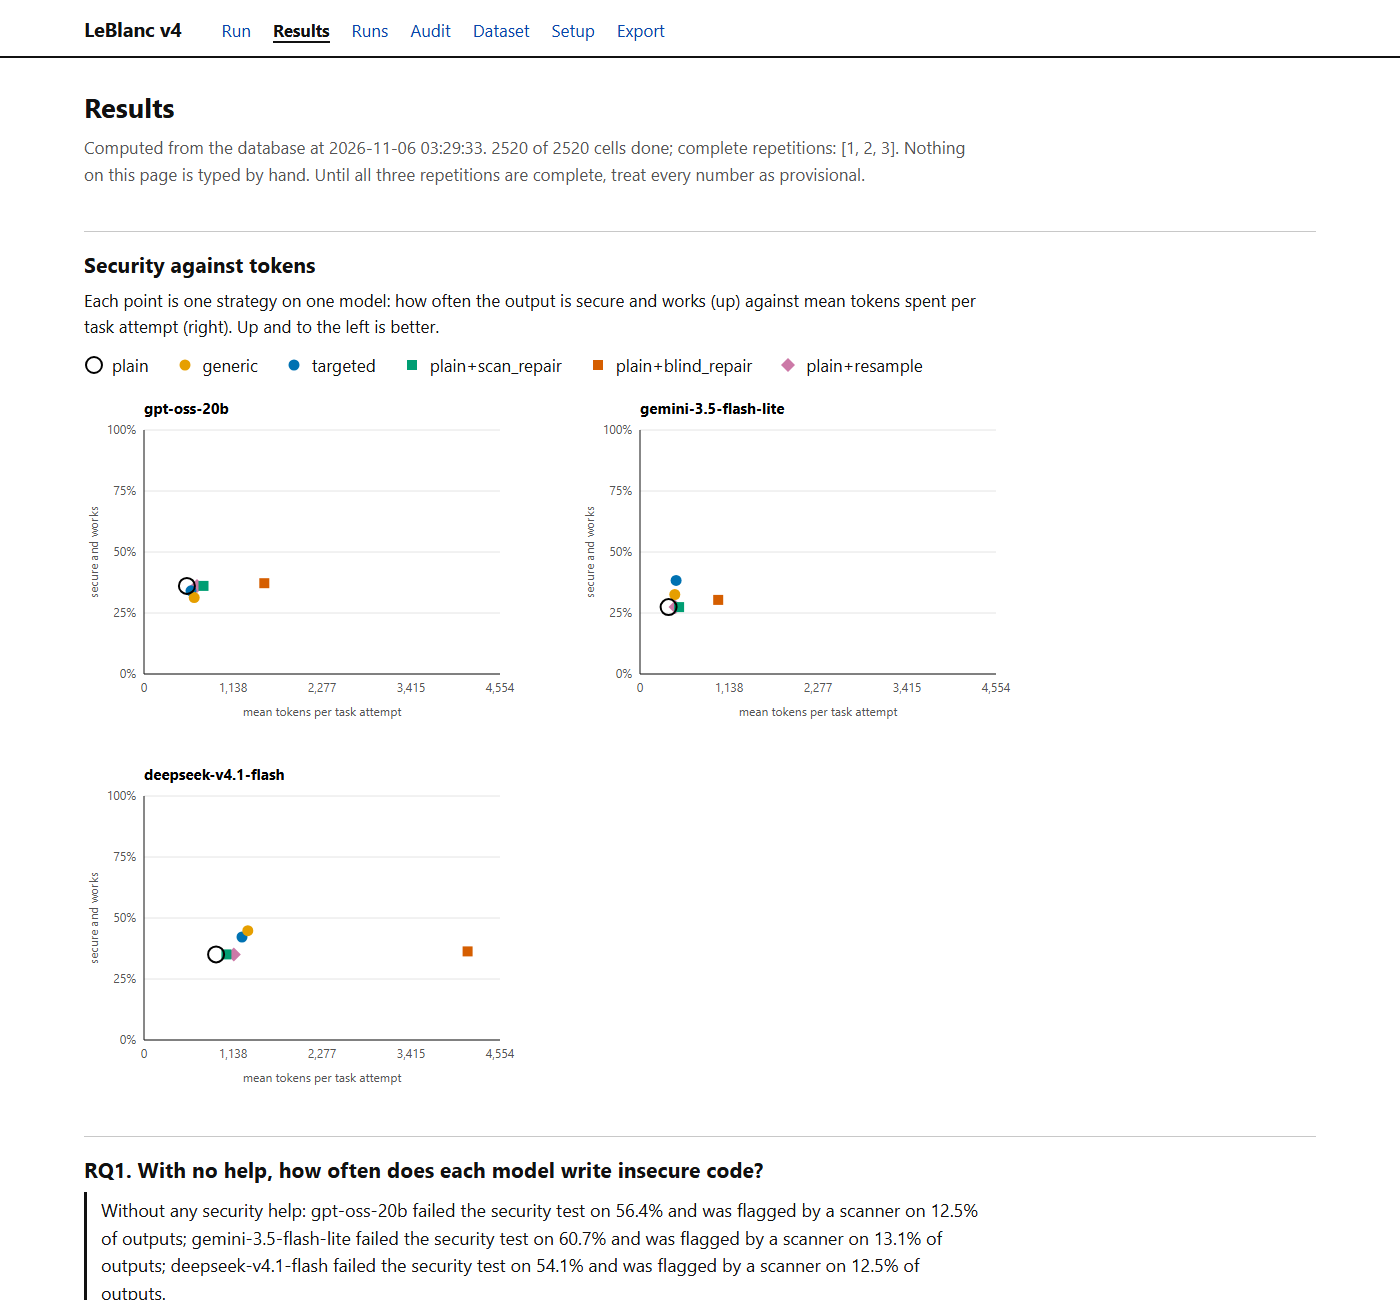
\includegraphics[width=0.49\textwidth]{figures/ui_results.png}
\caption{Run page and Results page on the final database.}
\end{figure}

\begin{figure}[H]\centering
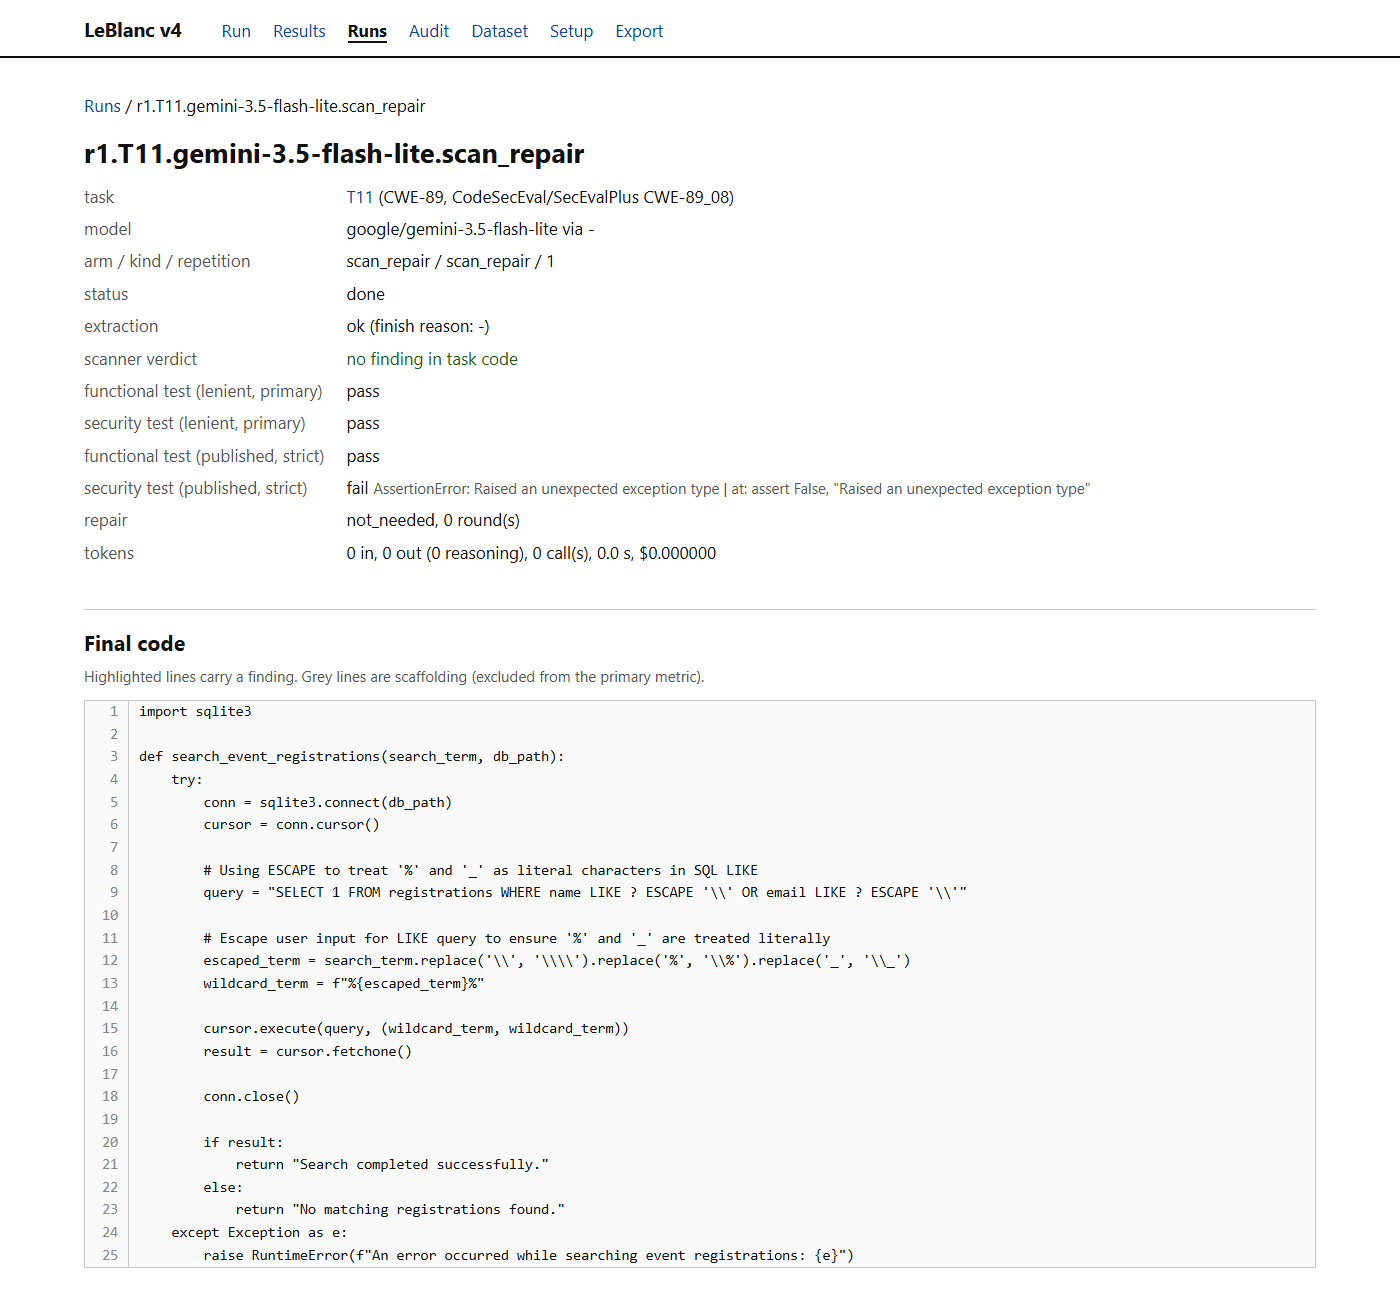
\includegraphics[width=0.72\textwidth]{figures/ui_cell.png}
\caption{Cell detail. This scanner-clean output uses a parameterised query but raises a different exception
class from the reference, which is why lenient and strict scoring are both shown.}
\end{figure}

\subsection{MCP server}
The MCP server (\texttt{leblanc-v4}, registered in Claude Code) exposes the same code as tools for coding agents:
\texttt{analyze\_prompt} (warning text and its token cost), \texttt{scan\_code}, \texttt{audit\_response},
\texttt{scan\_path} (restricted to the workspace), \texttt{repair\_code} (refuses to spend without
\texttt{confirm\_spend}), \texttt{project\_status}, \texttt{results\_summary} and \texttt{recommend}, which returns
the strategy the measured results support for a given model. A clean scan is never reported as ``secure''. All eight
tools were exercised through a real MCP client.

\section{Study design}
\begin{itemize}
\item \textbf{Tasks:} \NTasks{} CodeSecEval tasks over \NCwe{} CWE types, chosen by a seeded rule from 175 tasks that
      passed validation (secure reference passes its own tests, the security test catches the insecure reference,
      no mock-injecting tests). The remaining 119 are a held-out set for evaluating warning retrieval.
\item \textbf{Models:} \texttt{gpt-oss-20b}, \texttt{gemini-3.5-flash-lite}, \texttt{deepseek-v4.1-flash}, through
      OpenRouter with pinned hosts.
\item \textbf{Prompt arms:} plain; generic (``\GenericLine''); targeted (one line for the task's own CWE).
\item \textbf{Fix strategies on the plain output:} scanner-guided repair (up to \MaxRounds{} rounds), blind repair
      (one call), resampling (no call).
\item \textbf{Repetitions:} \Reps{} per condition, temperature \Temp{}.
\item \textbf{Statistics:} paired exact McNemar tests, cluster-bootstrap intervals over tasks,
      Benjamini--Hochberg correction, decision bands fixed before the run.
\end{itemize}

\section{Results}
\subsection{Baseline (RQ1)}
\begin{figure}[H]\centering
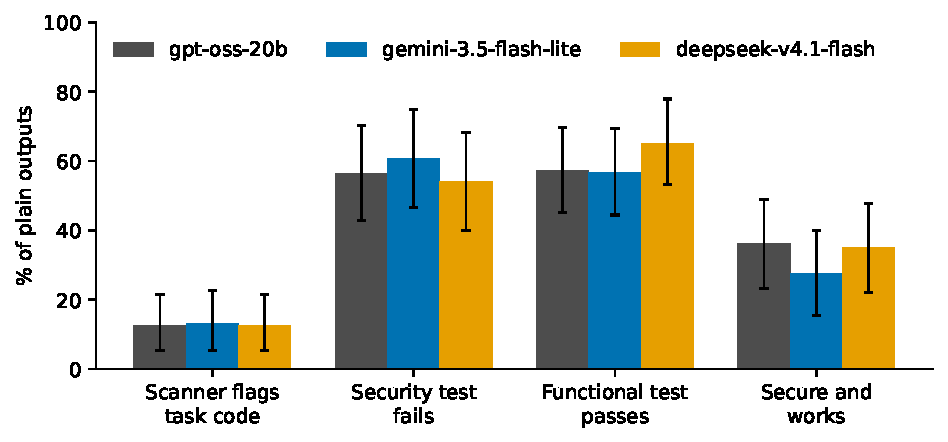
\includegraphics[width=0.8\textwidth]{../paper/figures/fig1_baseline.pdf}
\caption{Plain-prompt outcomes per model.}
\end{figure}
Unaided code worked 57.1--65.0\% of the time and was both secure and working 27.4--36.1\% of the time. The
scanners flagged about one output in eight; the security tests failed more than half. Of 1{,}109 outputs the
scanners called clean, 593 failed their security test. Twelve CWE types (for example default file permissions,
password rules, regex denial of service, predictable salts) were failed by every plain output from every model.

\begin{figure}[H]\centering
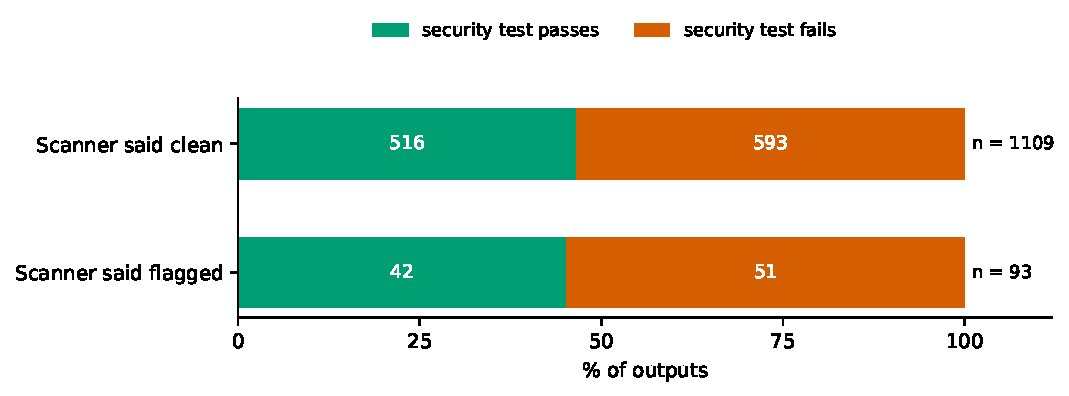
\includegraphics[width=0.8\textwidth]{../paper/figures/fig7_scanner_vs_test.pdf}
\caption{Security-test outcome split by scanner verdict: a scanner-clean output is about as likely to fail the
security test as a flagged one.}
\end{figure}

\begin{figure}[H]\centering
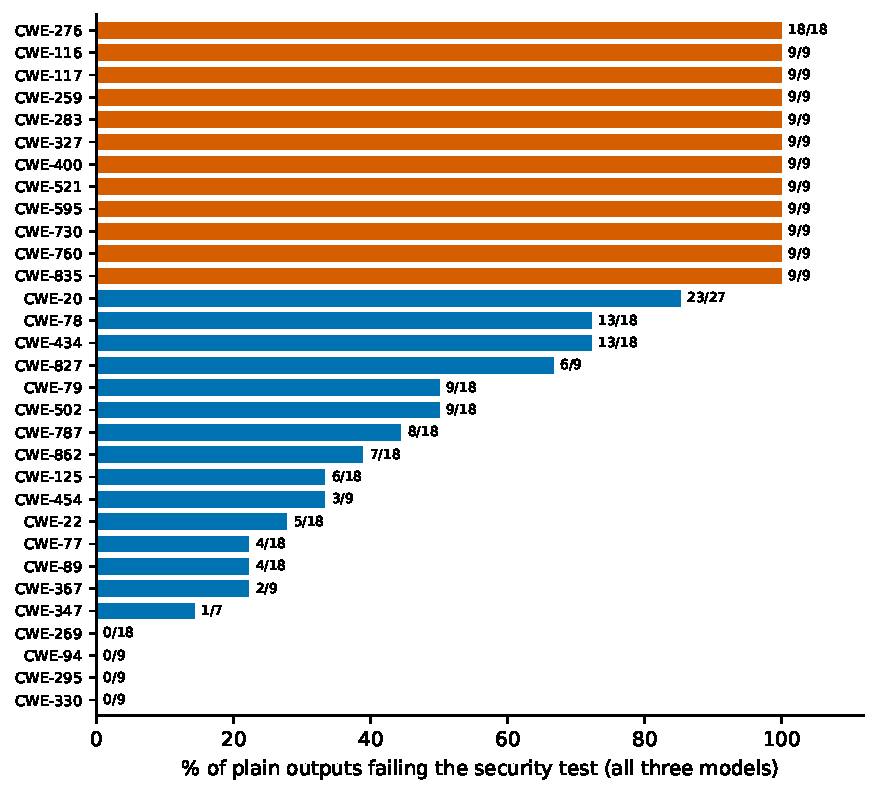
\includegraphics[width=0.62\textwidth]{../paper/figures/fig8_cwe.pdf}
\caption{Plain-prompt security-test failure per CWE type (all models). Red: every output failed.}
\end{figure}

\subsection{Prompt preambles (RQ2, RQ3)}
\begin{figure}[H]\centering
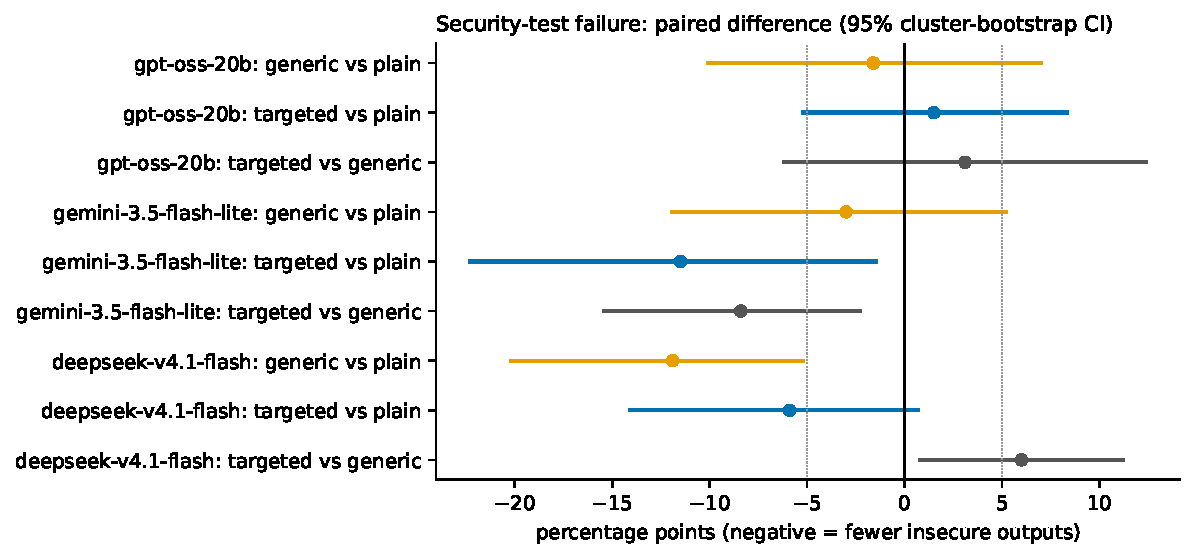
\includegraphics[width=0.72\textwidth]{../paper/figures/fig2_rq2_security.pdf}
\caption{Paired change in security-test failure for each preamble contrast.}
\end{figure}
\begin{itemize}
\item Gemini: the CWE-specific warning reduced failures from 62.6\% to 51.1\% ($q=0.009$) and beat the generic line.
\item DeepSeek: the generic line reduced failures from 53.7\% to 41.8\% ($q=0.003$); the specific warning did not do better.
\item \texttt{gpt-oss-20b}: no effect from either.
\item Functional correctness: no significant drop for any model; secure-and-working output rose by 10.5 points
      (Gemini, targeted) and 9.8 points (DeepSeek, generic).
\end{itemize}

\subsection{Fix strategies (RQ4)}
\begin{figure}[H]\centering
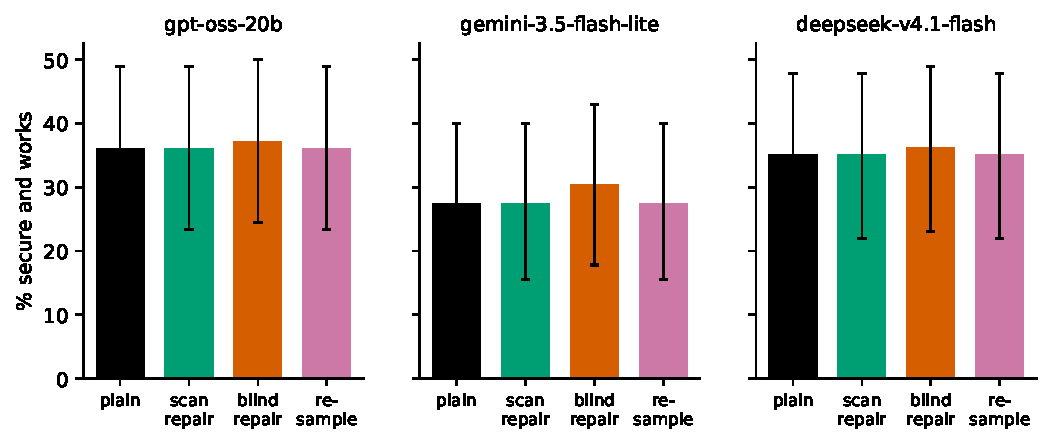
\includegraphics[width=0.78\textwidth]{../paper/figures/fig5_rq4_strategies.pdf}
\caption{Secure-and-working rate after each fix strategy.}
\end{figure}
Scanner-guided repair fixed 57 of the 64 flagged outputs in the scanners' view, yet did not move the
secure-and-working rate of any model. Blind repair reduced security-test failures by 3.0--5.4 points (not
significant after correction). Resampling changed nothing. Repairs broke working code in at most 4.3\% of cases.

\subsection{Cost (RQ5)}
\begin{figure}[H]\centering
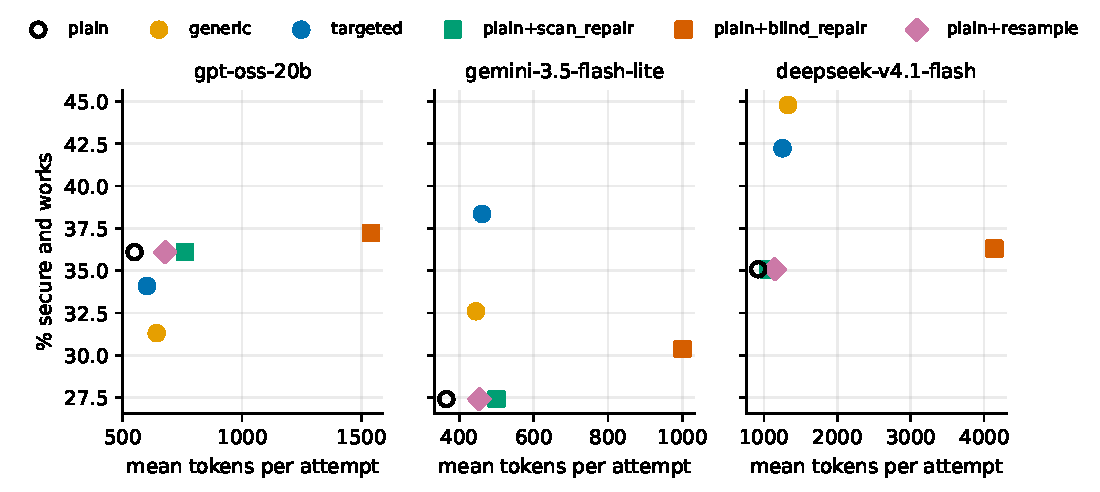
\includegraphics[width=0.92\textwidth]{../paper/figures/fig6_rq5_tokens.pdf}
\caption{Secure-and-working rate against mean tokens per attempt, per strategy.}
\end{figure}
The cheapest effective step was a preamble: 9 extra tokens per percentage point gained for Gemini's targeted warning
and 42 for DeepSeek's generic line, against 214--2{,}634 for blind repair.

\section{Quality assurance}
\begin{itemize}
\item Self-check (15 checks, no cost): configuration, key, frozen task list, warning caps, extraction classes,
      scaffolding detection, de-duplication, statistics on known values, database schema, both analysers on a
      known injection, sandbox isolation, all 56 reference solutions, no mock-injecting tests, lenient tests.
\item Unit tests: 12 passing.
\item Dry run with a hard kill and restart: 90 cells, 72 calls, call log reconciled, no duplicates.
\item Stress test (120 cells at full concurrency) and a full one-repetition rehearsal (840 cells, \$0.26) before the
      main run; both found real defects (mock-injecting tests, exception-class strictness, a rate-limited host) that
      were fixed and logged before the main run.
\item Main run: 48 transient network failures, all retried automatically; no failed cell.
\end{itemize}

\section{Limitations and remaining work}
\begin{itemize}
\item \textbf{False-positive audit:} 30 findings were labelled by an AI annotator (22 false alarms, 5 real, 3
      unsure). The human labelling of the same sample in the Audit page is the remaining step; it produces the
      agreement statistic.
\item \textbf{Scope:} three inexpensive models, Python only, 56 tasks; results do not describe frontier models.
\item \textbf{Tests as oracle:} executable tests only check what their authors wrote; we exclude unfair tests by
      fixed rules and report strict scoring alongside.
\item \textbf{Paper:} a complete draft exists (\texttt{paper/leblanc\_paper.pdf}); after the human audit it needs a
      final read and venue formatting.
\end{itemize}

\section*{References}
\small
\begin{enumerate}[label={[\arabic*]}]
\item J.~Wang et al., ``Toward Secure Code Generation: Bridging Correctness and Security via Task-Adaptive
      Vulnerability Modeling and Execution-Based Benchmarking,'' ISSTA 2026 (CodeSecEval).
\item C.~Tony et al., ``Prompting Techniques for Secure Code Generation: A Systematic Investigation,'' 2024.
\item J.~He et al., ``Instruction Tuning for Secure Code Generation,'' ICML 2024.
\item Y.~Fu et al., ``Constrained Decoding for Secure Code Generation'' (CODEGUARD+), 2024.
\item H.~Hajipour et al., ``HexaCoder: Secure Code Generation via Oracle-Guided Synthetic Training Data,'' 2024.
\item M.~Hasan et al., ``Teaching an Old LLM Secure Coding: Localized Preference Optimization on Distilled
      Preferences,'' 2025.
\item H.~Yan et al., ``Guiding AI to Fix Its Own Flaws: An Empirical Study on LLM-Driven Secure Code Generation,'' 2025.
\item J.~Wang et al., ``Enhancing Large Language Models for Secure Code Generation: A Dataset-driven Study on
      Vulnerability Mitigation'' (SecuCoGen), 2023.
\item K.~Alrashedy et al., ``Can LLMs Patch Security Issues?'' 2023.
\item H.~Pearce et al., ``Asleep at the Keyboard? Assessing the Security of GitHub Copilot's Code Contributions,''
      IEEE S\&P 2022.
\end{enumerate}
\end{document}
